\begin{inhalt}
\renewcommand*\chapterpagestyle{scrheadings}
\chapter{Gehäuse}

Für das Gehäuse wurde, wie in \ref{ref:fusion360_grundlagen} beschrieben, \texttt{Fusion 360} verwendet, um ein passendes Design zu erstellen.  
Um ein präzises Gehäuse zu konstruieren, sind einige vorbereitende Schritte notwendig.  
In diesem Fall wurde die Leiterplatte (PCB) aus \texttt{Altium Designer} als \texttt{STEP}-Datei exportiert und anschließend in \texttt{Fusion 360} importiert,  
um ein passgenaues Gehäuse um die Platine herum modellieren zu können.  
Hierfür wurde ein spezifischer Leitfaden verwendet \cite{artikel_pcb_way}.


\begin{figure}[!htb]
\centering
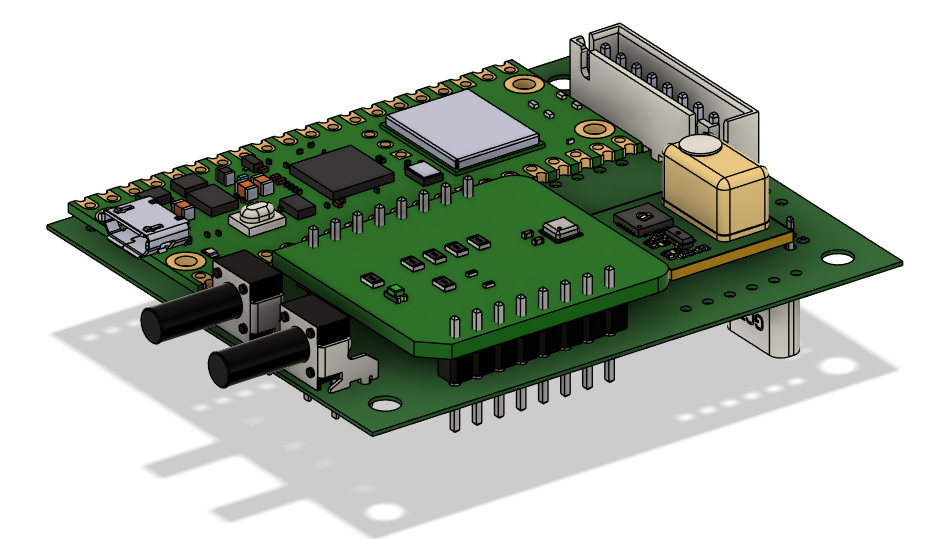
\includegraphics[width=0.65\textwidth]{files/Thomas/pics/geheause/pcb_fusion.png}
\caption[Bildbezeichnung für Abbildungsverzeichnis]{}
\label{fig:pcb_v2}
\end{figure}


Außerdem wurde das Displaymodell von einer Website \cite{3d_display_website} heruntergeladen und in das Projekt integriert.


\begin{figure}[!htb]
\centering
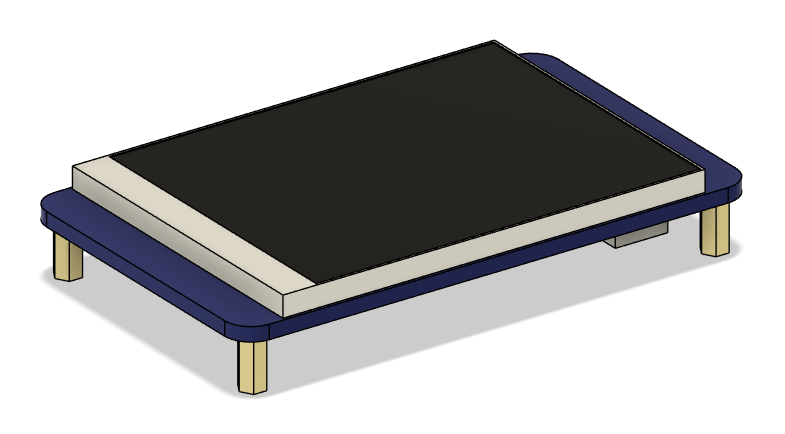
\includegraphics[width=0.55\textwidth]{files/Thomas/pics/geheause/display_fusion.png}
\caption[Bildbezeichnung für Abbildungsverzeichnis]{}
\label{fig:display_3d}
\end{figure}

\clearpage

\section{Version 1.0}
\label{ref:gehaeuse_1_0}

\begin{figure}[!htb]
\centering
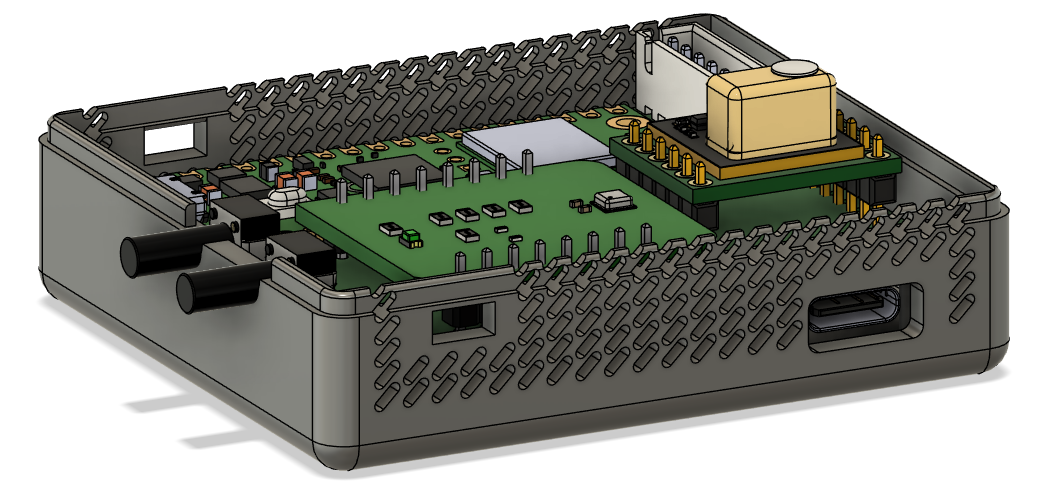
\includegraphics[width=0.45\textwidth]{files/Thomas/pics/geheause/1.0/gehaeuse_side.png}
\caption[Bildbezeichnung für Abbildungsverzeichnis]{}
\label{fig:gehaeuse_side_v1_0}
\end{figure}

Beim ersten Meilenstein traten noch zahlreiche Probleme auf. Wie in der Abbildung \ref{fig:gehaeuse_side_v1_0} ersichtlich, basierte diese Version auf der \texttt{PCB} Version 1.0 (\ref{ref:PCB_Version_1}).  
Besonders problematisch war der USB-C-Port an der Seite der Platine. Da dieser sehr nah am Rand der \texttt{PCB} positioniert war und USB-C-Kabel nicht genormte Gehäusegrößen besitzen,  
musste ein besonders großes Loch in das Gehäuse eingeplant werden, um mit allen Steckern kompatibel zu sein.  

\vspace{0.15cm}

Außerdem wurden in der Front nur zwei Clips verwendet, was sich jedoch als unzureichend herausstellte.  


\vspace{0.15cm}

Für einen optimierten Airflow wurde dasselbe Lüftungsmuster verwendet, das zuvor durch Internetrecherche identifiziert wurde.



\begin{figure}[!htb]
\centering
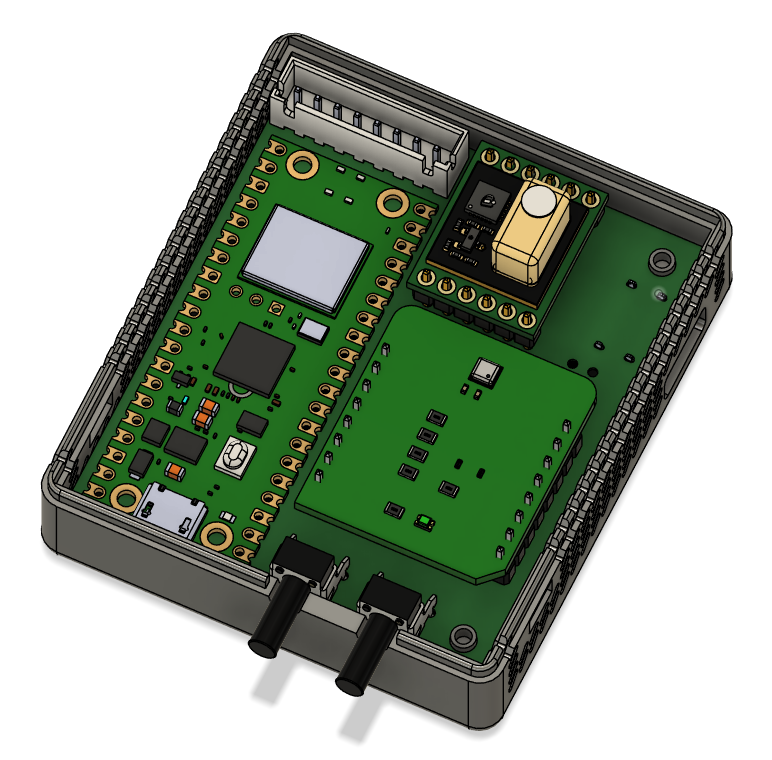
\includegraphics[width=0.4\textwidth]{files/Thomas/pics/geheause/1.0/gehaeuse_top.png}
\caption[Bildbezeichnung für Abbildungsverzeichnis]{}
\label{fig:gehaeuse_top_1_0}
\end{figure}


Wie in Abbildung \ref{fig:gehaeuse_top_1_0} zu erkennen ist, waren bei der ersten Version die Wandstärken des Gehäuses sehr gering, wodurch die dünneren Bereiche bei jeder Belastung leicht abbrachen.



\vspace{0.15cm}

Außerdem passte das Display im oberen Teil des Gehäuses noch nicht vollständig.

\newpage

\section{Version 1.1}

\begin{figure}[!htb]
\centering
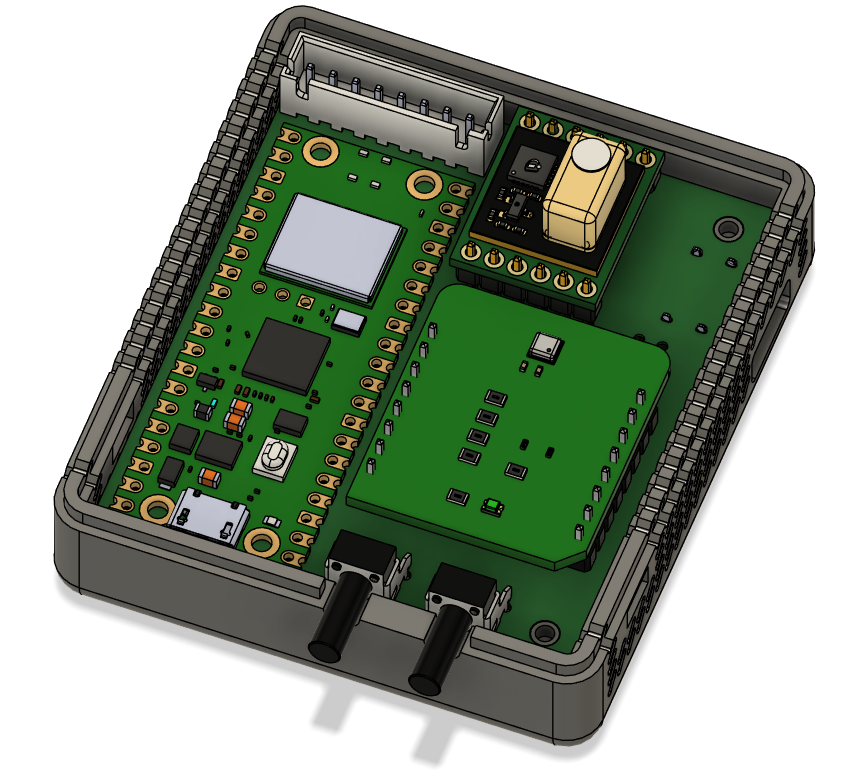
\includegraphics[width=0.55\textwidth]{files/Thomas/pics/geheause/1.1/gehaeuse_top.png}
\caption[Bildbezeichnung für Abbildungsverzeichnis]{}
\label{fig:gehaeuse_internet_bild}
\end{figure}

Der wesentliche Unterschied zwischen Version 1.0 (Zu sehen in: \ref{ref:gehaeuse_1_0}) und 1.1 besteht darin, dass die Seitenwände des Gehäuses verstärkt wurden, um eine höhere Stabilität zu gewährleisten und ein leichtes Brechen zu verhindern.

\newpage

\section{Version 1.2}

\begin{figure}[!htb]
\centering
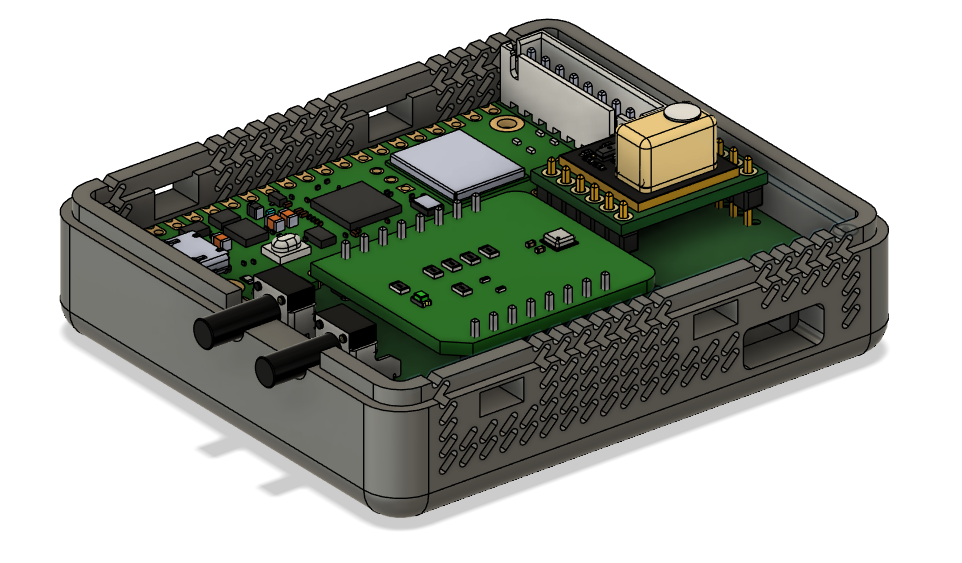
\includegraphics[width=0.6\textwidth]{files/Thomas/pics/geheause/1.2/gehaeuse_side.png}
\caption[Bildbezeichnung für Abbildungsverzeichnis]{}
\label{fig:gehaeuse_internet_bild}
\end{figure}

In dieser Version wurden zwei zusätzliche Clips hinzugefügt, um den Verschlussmechanismus zu verbessern.  
Ohne diese Ergänzung hätte sich das Gehäuse zu leicht öffnen lassen.

\vspace{1cm}

\begin{figure}[!htb]
\centering
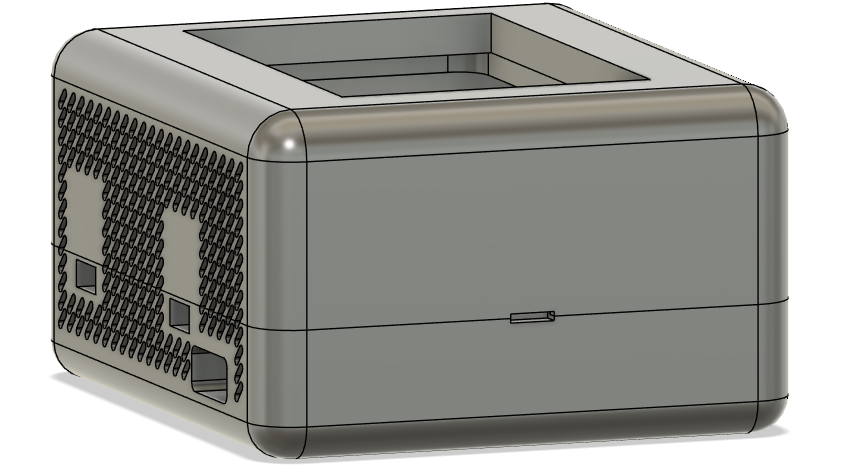
\includegraphics[width=0.6\textwidth]{files/Thomas/pics/geheause/1.2/gehaeuse_back.png}
\caption[Bildbezeichnung für Abbildungsverzeichnis]{}
\label{fig:gehaeuse_internet_bild}
\end{figure}

Außerdem wurde nun wenn das gehäuse zu stereng aufgeht ein Schlitz zwischen den Obrigen teil und den untrigen Teil gemacht um zu garantiren das man mit einen Schlitzschraufenziher das gehäuse aufzuamachen können.

\vspace{0.15cm}

Zudem wurde die Aussparung für das Display optimiert, sodass es nun passgenau mit den erforderlichen Toleranzen und allen notwendigen Anpassungen in das Gehäuse eingesetzt werden kann.

\newpage

\section{Version 2.0}

\begin{figure}[!htb]
\centering
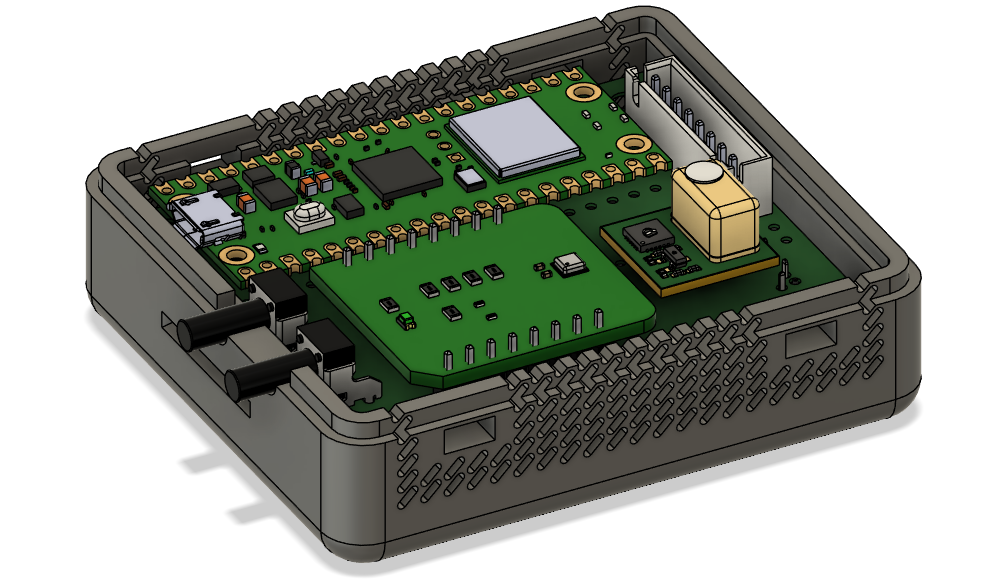
\includegraphics[width=0.6\textwidth]{files/Thomas/pics/geheause/2.0/gehaeuse_side.png}
\caption[Bildbezeichnung für Abbildungsverzeichnis]{}
\label{fig:gehaeuse_internet_bild}
\end{figure}

Nachdem die \texttt{PCB} Version 2 (Siehe auf: \ref{ref:PCB_Version_2}) fertiggestellt war, wurde das Gehäuse neu designt, um erneut zur Platine zu passen.  
Ein wesentlicher Vorteil dieser Version besteht darin, dass sich der USB-C-Anschluss nicht mehr seitlich befindet.  
Dadurch konnten die Clips symmetrisch und in gleichem Abstand zur Gehäusemitte positioniert werden, was eine deutlich stabilere Verbindung zwischen den Gehäuseteilen ermöglicht.
 

\vspace{0.15cm}

Zusätzlich wurden kleine Schlitze in das Gehäuse integriert, um die Montage im Kabelkanal der Schulräume der HTL St. Pölten zu erleichtern.  
Diese Schlitze ermöglichen es, das Gerät einfach in den dafür vorgesehenen Adapter einzustecken.


\begin{figure}[!htb]
\centering
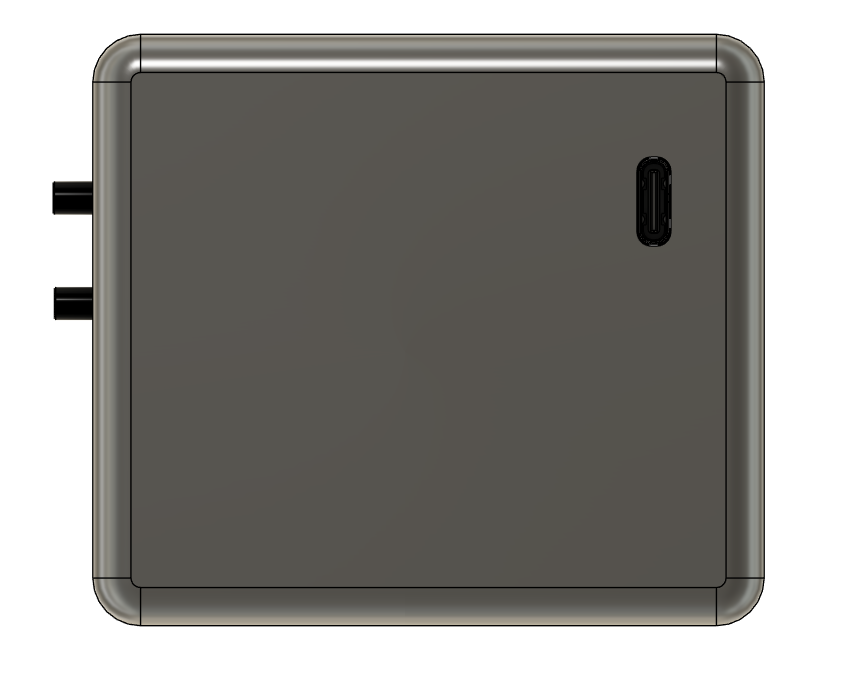
\includegraphics[width=0.5\textwidth]{files/Thomas/pics/geheause/2.0/gehaeuse_bot.png}
\caption[Bildbezeichnung für Abbildungsverzeichnis]{}
\label{fig:gehaeuse_internet_bild}
\end{figure}

Da sich der USB-C-Anschluss nun nicht mehr an der Seite, sondern an der Unterseite des Gehäuses befindet, entfällt das Problem unterschiedlicher USB-C-Steckergrößen.  
Somit ist gewährleistet, dass sämtliche USB-C-Kabel problemlos passen.


\section{Version 2.1}

\begin{figure}[!htb]
\centering
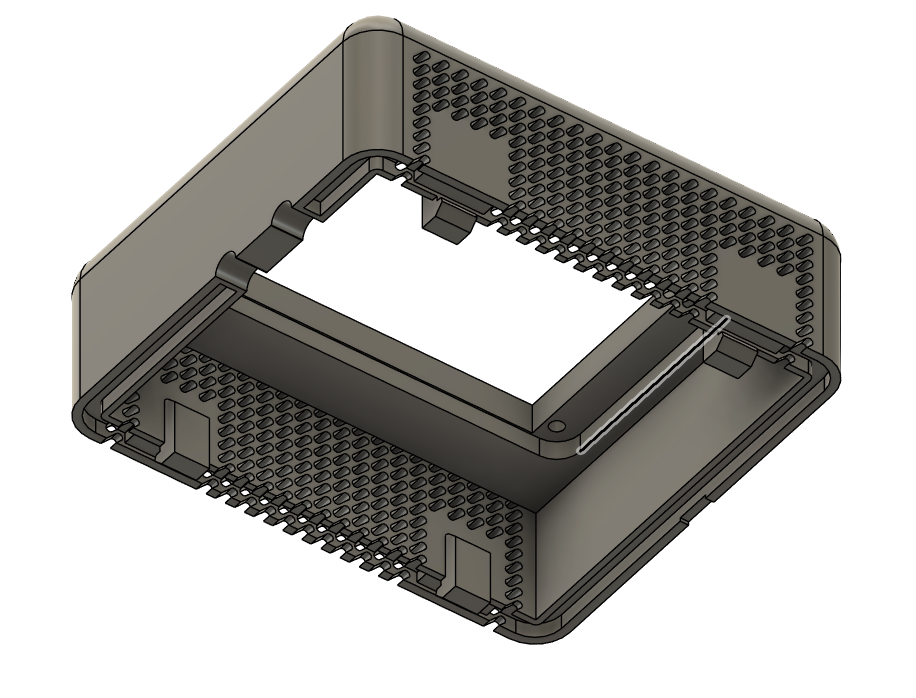
\includegraphics[width=0.65\textwidth]{files/Thomas/pics/geheause/2.1/gehaeuse_side.png}
\caption[Bildbezeichnung für Abbildungsverzeichnis]{}
\label{fig:gehaeuse_internet_bild}
\end{figure}



Da die Clips wiederholt Probleme verursachten, wurden sie im Inneren verstärkt.  
Zudem wurden sie verkleinert, um Konflikte mit der Gehäusedicke zu vermeiden.


\newpage

\section{Adapter für Kabelkanal}

Für die Installation des ClassScouts in den Klassenräumen wurde ein spezieller Adapter entworfen, der dafür vorgesehen ist, im Kabelkanal der HTL St. Pölten montiert zu werden.


\subsection{Version 1.0}

In der ersten Version wurde probiert einfach die Mase des Kabelkanals zu Treffen und zu schauen das die Knöpfe drückbar sind von außen.

\begin{figure}[!htb]
\centering
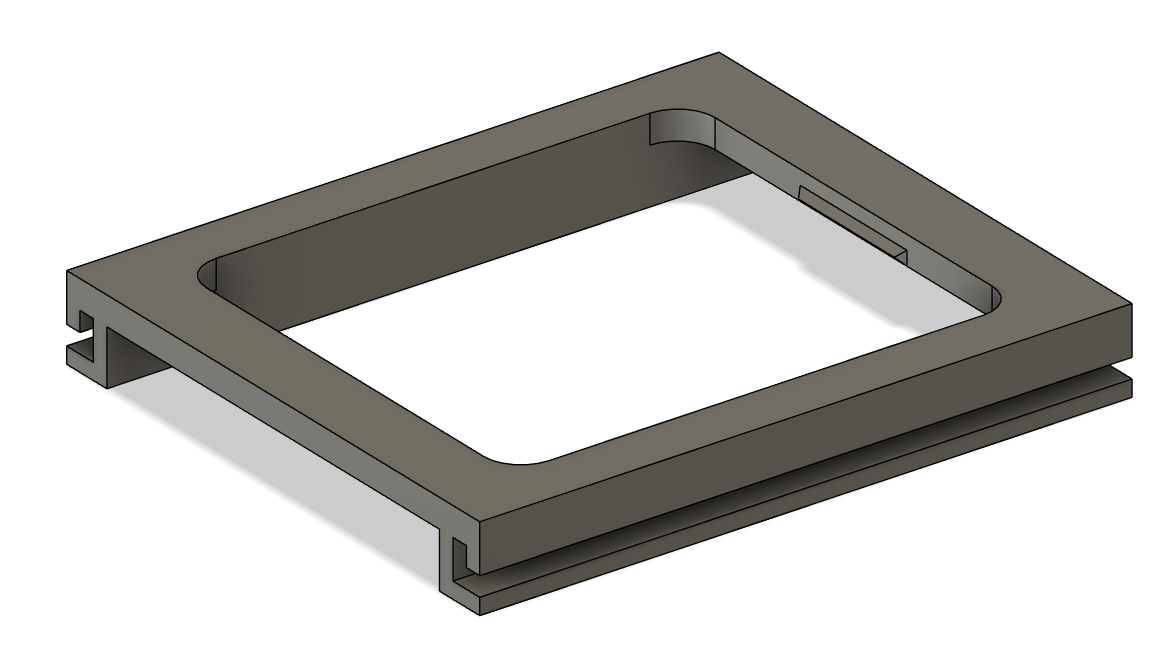
\includegraphics[width=0.5\textwidth]{files/Thomas/pics/adapter/1.0/image.png}
\caption[Bildbezeichnung für Abbildungsverzeichnis]{}
\label{fig:gehaeuse_internet_bild}
\end{figure}


\subsection{Version 2.0}

In Version 2 wurde eine Öffnung für ein USB-C-Kabel hinzugefügt, sodass dieses nun von außen in den Kabelkanal geführt werden kann.  
Zudem wurden die Toleranzen optimiert, um den Einbau des Gehäuses zu erleichtern.


\begin{figure}[!htb]
\centering
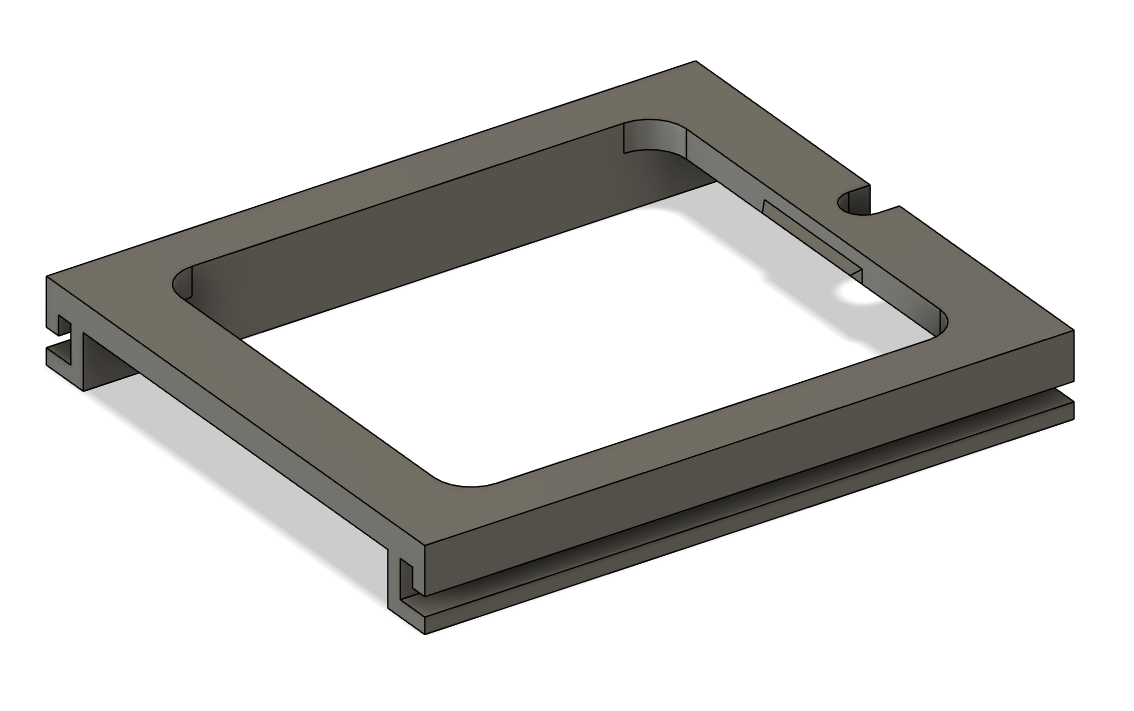
\includegraphics[width=0.55\textwidth]{files/Thomas/pics/adapter/2.0/image.png}
\caption[Bildbezeichnung für Abbildungsverzeichnis]{}
\label{fig:gehaeuse_internet_bild}
\end{figure}



\section{Slicen und 3D-Druck}

Da bei einem FDM-3D-Drucker Schicht für Schicht aufgebaut wird, entstehen leicht geradlinige Bruchstellen.  
Besonders problematisch war dies bei den Clips, die das Gehäuse zusammenhalten sollten.  
Nach längerem Ausprobieren wies ein Klassenkollege darauf hin, dass sich das Problem durch das Drucken des Gehäuses in einem Winkel von 45° lösen ließe.  
Durch diese Ausrichtung verlaufen die Schichten schräg, wodurch sie sich nicht so leicht voneinander trennen und die Clips deutlich stabiler werden.  
Diese Methode wurde umgesetzt und das Problem erfolgreich behoben.


\begin{figure}[!htb]
\centering
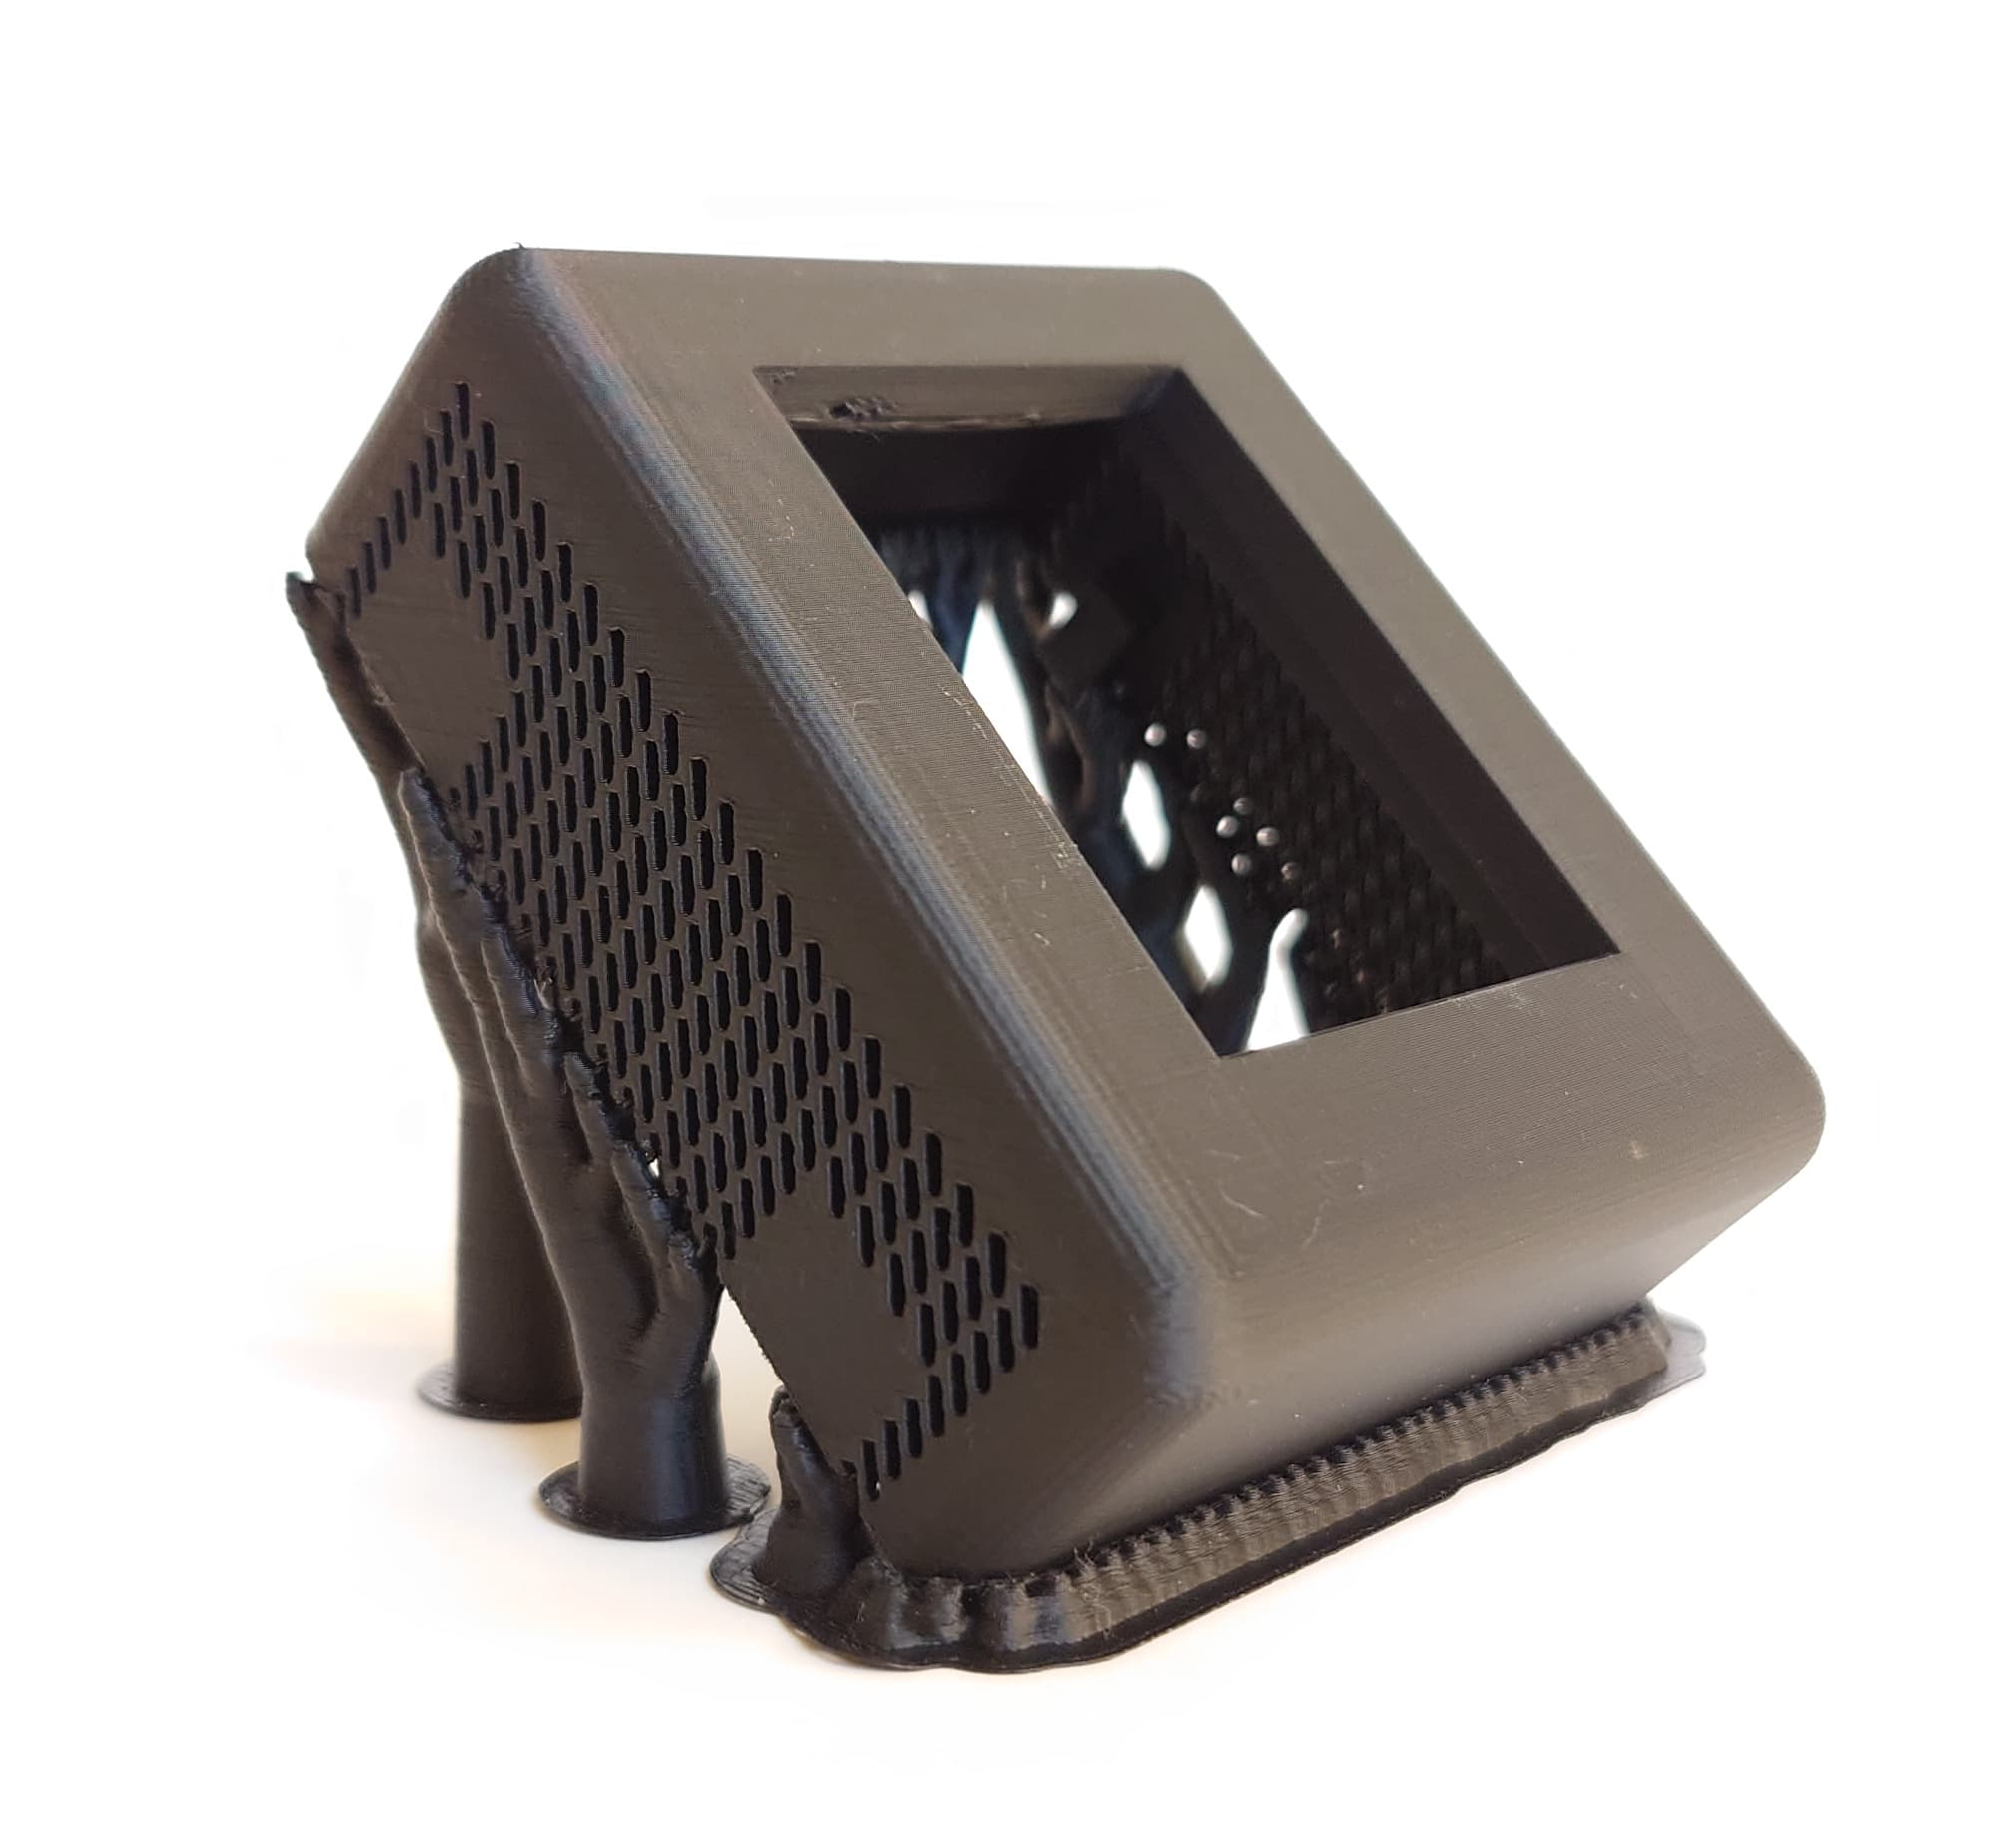
\includegraphics[width=0.75\textwidth]{files/Thomas/pics/geheause/gehaeuese_45_Grad_druck.png}
\caption[Bildbezeichnung für Abbildungsverzeichnis]{}
\label{fig:gehaeuse_internet_bild}
\end{figure}

Das Gehäuse wurde mit einem \texttt{Bambu Lab A1} FDM-3D-Drucker gefertigt und zuvor mit dem \texttt{Bambu Slicer} gesliced, um einen optimalen G-Code zu generieren.  
Die Clips wurden mit einer Füllung von 100\% gedruckt, während der restliche Teil des Gehäuses mit einer Füllung von 20\% gedruckt wurde.  
Zudem musste das Gehäuse mit einer Schichthöhe von 0{,}1\,mm gedruckt werden, um das Lüftungsmuster korrekt zu drucken.


\end{inhalt}